\chapter{El semiplano superior}
\label{cap:semiplano-superior}

Otro modelo plano del espacio hiperbólico es el semiplano superior
\[
  \mathbb{H}=\{x+iy\in\mathbb{C}:y>0\},
\]
equipado con la métrica
\begin{equation}
  ds^2=\frac{dx^2+dy^2}{y^2}.
  \label{eq:metrica-semiplano}
\end{equation}
La frontera ideal es el eje real junto con el punto al infinito. Una figura queda guardada como código TikZ en \texttt{assets/tikz/semiplano-superior} y se inserta con \verb|\input|, igual que la del \cref{cap:disco-poincare}.

\section{Geodésicas y longitud}

Las geodésicas son las rectas verticales y las semicircunferencias cuyos centros están sobre el eje real. La \cref{fig:semiplano-superior} muestra ambas formas. La longitud de una curva parametrizada \((x(t),y(t))\) se calcula con
\[
  L=\int \frac{\sqrt{x'(t)^2+y'(t)^2}}{y(t)}\,dt.
\]
El factor \(1/y\) hace que las distancias se compriman en coordenadas euclidianas al subir por el semiplano.

\begin{figure}[htbp]
  \centering
  % Fragmento reutilizable: las geodésicas son verticales o semicircunferencias.
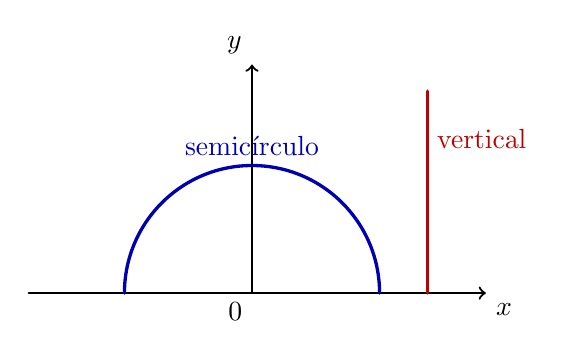
\begin{tikzpicture}[scale=1.35,line cap=round]
  \draw[->,thick] (-2.1,0) -- (2.2,0) node[below right] {$x$};
  \draw[->,thick] (0,0) -- (0,2.15) node[above left] {$y$};
  \draw[blue!70!black,very thick] (-1.2,0)
    arc[start angle=180,end angle=0,radius=1.2cm];
  \draw[red!75!black,very thick] (1.65,0) -- (1.65,1.9);
  \node[blue!70!black,above] at (0,1.2) {semicírculo};
  \node[red!75!black,right] at (1.65,1.45) {vertical};
  \node[below left] at (0,0) {$0$};
\end{tikzpicture}

  \caption{Una geodésica vertical y una semicircunferencia ortogonal al eje real.}
  \label{fig:semiplano-superior}
\end{figure}

\section{Transformaciones de Möbius}

Las matrices reales
\[
  \begin{pmatrix}a&b\\c&d\end{pmatrix},
  \qquad ad-bc=1,
\]
actúan mediante
\[
  z\longmapsto\frac{az+b}{cz+d}.
\]
Estas transformaciones preservan el semiplano y su métrica. Identificando matrices que difieren por un signo, el grupo resultante se denota \(\mathrm{PSL}(2,\mathbb{R})\). Esta acción permite mover puntos y geodésicas a posiciones convenientes para los cálculos \cite{anderson2005}.

\section{Relación con el disco}

La transformación de Cayley
\[
  \phi(z)=i\frac{1+z}{1-z}
\]
lleva el disco unitario al semiplano superior y preserva la métrica hiperbólica. En los dos dibujos, las fronteras representan puntos ideales y no pertenecen al plano hiperbólico. Los modelos describen la misma geometría con coordenadas distintas.
